%-------------------------------------------------------------------------------
% This file provides a skeleton ATLAS note.
% \pdfinclusioncopyfonts=1
% This command may be needed in order to get \ell in PDF plots to appear. Found in
% https://tex.stackexchange.com/questions/322010/pdflatex-glyph-undefined-symbols-disappear-from-included-pdf
%-------------------------------------------------------------------------------
% Specify where ATLAS LaTeX style files can be found.
\newcommand*{\ATLASLATEXPATH}{latex/}
% Use this variant if the files are in a central location, e.g. $HOME/texmf.
% \newcommand*{\ATLASLATEXPATH}{}
%-------------------------------------------------------------------------------
\documentclass[NOTE, atlasdraft=true, texlive=2016, UKenglish]{\ATLASLATEXPATH atlasdoc}
\usepackage{float}
\usepackage{euler}\usepackage{pgf}
%\usepackage{subcaption}
%\usepackage{natbib}
\usepackage{geometry}
\usepackage{pdflscape}
\usepackage{setspace}
%\setstretch{2}
%\setlength{\parindent}{1cm}
\usepackage{chngcntr}
\counterwithin{figure}{section}
\counterwithin{equation}{section}
% The language of the document must be set: usually UKenglish or USenglish.
% british and american also work!
% Commonly used options:
%  atlasdraft=true|false This document is an ATLAS draft.
%  texlive=YYYY          Specify TeX Live version (2016 is default).
%  coverpage             Create ATLAS draft cover page for collaboration circulation.
%                        See atlas-draft-cover.tex for a list of variables that should be defined.
%  cernpreprint          Create front page for a CERN preprint.
%                        See atlas-preprint-cover.tex for a list of variables that should be defined.
%  NOTE                  The document is an ATLAS note (draft).
%  PAPER                 The document is an ATLAS paper (draft).
%  CONF                  The document is a CONF note (draft).
%  PUB                   The document is a PUB note (draft).
%  BOOK                  The document is of book form, like an LOI or TDR (draft)
%  txfonts=true|false    Use txfonts rather than the default newtx
%  paper=a4|letter       Set paper size to A4 (default) or letter.

%-------------------------------------------------------------------------------
% Extra packages:
%\usepackage{\ATLASLATEXPATH atlaspackage}
\usepackage[subfigure]{\ATLASLATEXPATH atlaspackage} 
% Commonly used options:
%  biblatex=true|false   Use biblatex (default) or bibtex for the bibliography.
%  backend=bibtex        Use the bibtex backend rather than biber.
%  subfigure|subfig|subcaption  to use one of these packages for figures in figures.
%  minimal               Minimal set of packages.
%  default               Standard set of packages.
%  full                  Full set of packages.
%-------------------------------------------------------------------------------
% Style file with biblatex options for ATLAS documents.
\usepackage{\ATLASLATEXPATH atlasbiblatex}

% Package for creating list of authors and contributors to the analysis.
\usepackage{\ATLASLATEXPATH atlascontribute}

% Useful macros
\usepackage{\ATLASLATEXPATH atlasphysics}
% See doc/atlas_physics.pdf for a list of the defined symbols.
% Default options are:
%   true:  journal, misc, particle, unit, xref
%   false: BSM, heppparticle, hepprocess, hion, jetetmiss, math, process, other, texmf
% See the package for details on the options.

% Files with references for use with biblatex.
% Note that biber gives an error if it finds empty bib files.
%\addbibresource{ttHDiff.bib}
\addbibresource{bib/higgsDiffNote.bib}
\addbibresource{bib/wz_int_note.bib}
\addbibresource{bib/ATLAS.bib}
\addbibresource{bib/CMS.bib}
\addbibresource{bib/ConfNotes.bib}
\addbibresource{bib/PubNotes.bib}

% Paths for figures - do not forget the / at the end of the directory name.
\graphicspath{{logos/}{figures/}}

% Add you own definitions here (file wz_heavy_flavor-defs.sty).
\usepackage{ttHDiff-defs}

%-------------------------------------------------------------------------------
% Generic document information
%-------------------------------------------------------------------------------

% Title, abstract and document 
\input{ttHDiff-metadata}
% Author and title for the PDF file
\hypersetup{pdftitle={ATLAS document},pdfauthor={The ATLAS Collaboration}}

%\renewcommand{\baselinestretch}{2}

%-------------------------------------------------------------------------------
% Content
%-------------------------------------------------------------------------------
\begin{document}

\maketitle

\begin{singlespace}
\tableofcontents
\end{singlespace}

% List of contributors - print here or after the Bibliography.
%\PrintAtlasContribute{0.30}
\clearpage

%------------------------------------------------------------------------------
\section{Changes and outstanding items}
\label{sec:changes}
%------------------------------------------------------------------------------

\subsection{Changelog}

This is version 1

\clearpage
%-------------------------------------------------------------------------------

%-------------------------------------------------------------------------------
\section{Introduction}
\label{sec:intro}
Since the discovery of a Higgs boson compatable with the Standard Model (SM) in 2012 \cite{HIGG-2011-02}, its interactions with other particles have been studied using proton-proton collision data produced by the Large Hadron Collider (LHC). The strongest of these interactions is the coupling of the Higgs to the top quark, making the Yukawa coupling between these two particles of particular interest for study.

These interactions can be measured directly by studying the production of a Higgs Boson in association with a pair of Top Quarks ($t\bar{t}H$). While this process has been observed by both the ATLAS and CMS collaborations, these analyses have focused on measuring the overall rate of $t\bar{t}H$ production. There are several theories of physics Beyond the Standard Model (BSM), however, that would affect the kinematics involved in $t\bar{t}H$ production without altering its overall rate \cite{Dumont_2013}.  

An Effective Field Theory approach can be used to model the low energy effects of new, high energy physics, by paramaterizing BSM effects as dimension-six operators. The addition of these operators can be shown to modify the transverse momentum ($p_T$) spectrum of the Higgs Boson \cite{Banerjee_2014}. Therefore, reconstructing the momentum spectrum of the Higgs provides a means to observe new physics in the Higgs sector.  

This note reports on the feasability of performing differential measurements in $t\bar{t}H$ events with multiple leptons in the final state, using Monte Carlo (MC) simulations scaled to 139 $fb^{-1}$ at an energy $\sqrt{s} = 13$ TeV. Events are separated into channels based on the number of light leptons (electrons and muons) in the final state - either two same-sign leptons ($2lSS$), or three leptons ($3l$), where the $3l$ channel is split into two based on the decay of the Higgs.

The presence of multiple neutrinos in the final state of the multilepton channels introduces an ambiguity that prevents the Higgs from being fully recontructed. This motivates the use of sophisticated machine learning techniques to better predict the Higgs \pt spectrum for these events. A deep neural network is used to identify which objects originate from the decay of the Higgs, and reconstruct the momentum of the Higgs Boson in each event. This spectrum is fit to data in the three decay channels considered in order to extract normalization factors on $t\bar{t}H$ produced with high ($>150$ GeV) and low ($<150$ GeV) Higgs.

This note is organized as follows: The dataset and Monte Carlo (MC) simulations used in the analysis is outlined in Section \ref{sec:dataMC}. Section \ref{sec:objReco} describes the identification and reconstruction of the various physics objects. The models used to reconstruct the momentum spectrum of the Higgs is discussed in Section \ref{sec:mva}. The selection and categorisation of events comprises Section \ref{sec:signal_region}, and the theoritical and experimental systematic uncertainties considered are described in Section \ref{sec:sys}. Finally, the results of the study are summarized in Section \ref{sec:results}.

%-------------------------------------------------------------------------------

%-------------------------------------------------------------------------------
%\section{The ATLAS Detector}
%\label{sec:ATLAS}
%ATLAS (a not terribly natural acronym for ``A Toroidal LHC Apparatus'') is a general purpose detector designed to maximize the detection efficiency of all physics objects, including leptons, jets, and photons. This means it is capable of measuring all SM particles, with the exception of neutrinos, the presence of which can be inferred based on missing transverse momentum. The detector measures 44 m long, and 25 m tall. 

The ATLAS detector consists of multiple layers, each of which serves a different purpose in reconstructing collisions. At the very center of the detector is the interaction point where the proton beams of the LHC collide. 

\begin{figure}[H]
\centering
   \includegraphics[width=0.75\linewidth]{figures/lhc/ATLASdiagram.eps}
\caption{Cutaway view of the ATLAS detector, with labels of its major components \cite{ATLAS_figure}.}
\label{fig:ATLAS}
\end{figure}

\subsection{Inner Detector}
\label{sec:innerDetector}

\begin{figure}[H]
\centering
   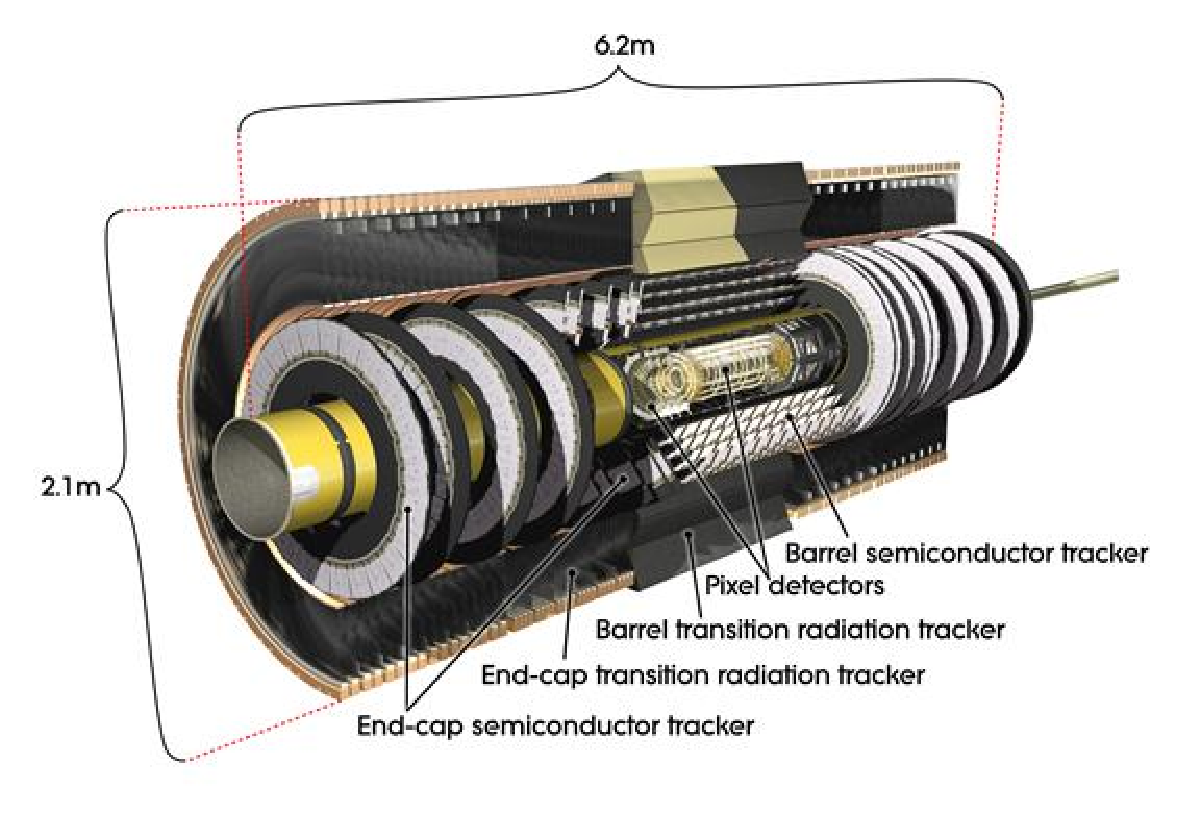
\includegraphics[width=0.75\linewidth]{figures/lhc/InnerDetector.eps}
\caption{Cutaway view of the Inner Detector \cite{caloFig}.}
\label{fig:innerDect}
\end{figure}

Just surrounding the interaction point is the Inner Detector, designed to track the path of charged particles moving through the detector. An inner solenoid surrounding the Innder Detector is used to produces a magnetic field of 2 T. This large magnetic field causes the path of charged particles moving through the Inner Detector to bend. Because this magnetic field is uniform and well known, it can be used in conjunction with the curvature of a particles path to measure its charge and momentum.

The Inner Detector consists of three components - the Pixel Detector, the Semi-Conductor Tracker (SCT), and the Transition Radiation Tracker (TRT). The Pixel Detector is the innermost of these, beginning just 33.25 mm away from the beam line. It consists of three silicon layers along the barrel, as well as three endcap layers, covering a range of $|\eta|$ < 2.5. 

The Semiconductor Tracker (SCT) is similar to the Pixel detector, but uses long strips rather than small pixel to cover a larger spatial area.

\subsection{Calorimeters}
\label{sec:calo}

\begin{figure}[H]
\centering
   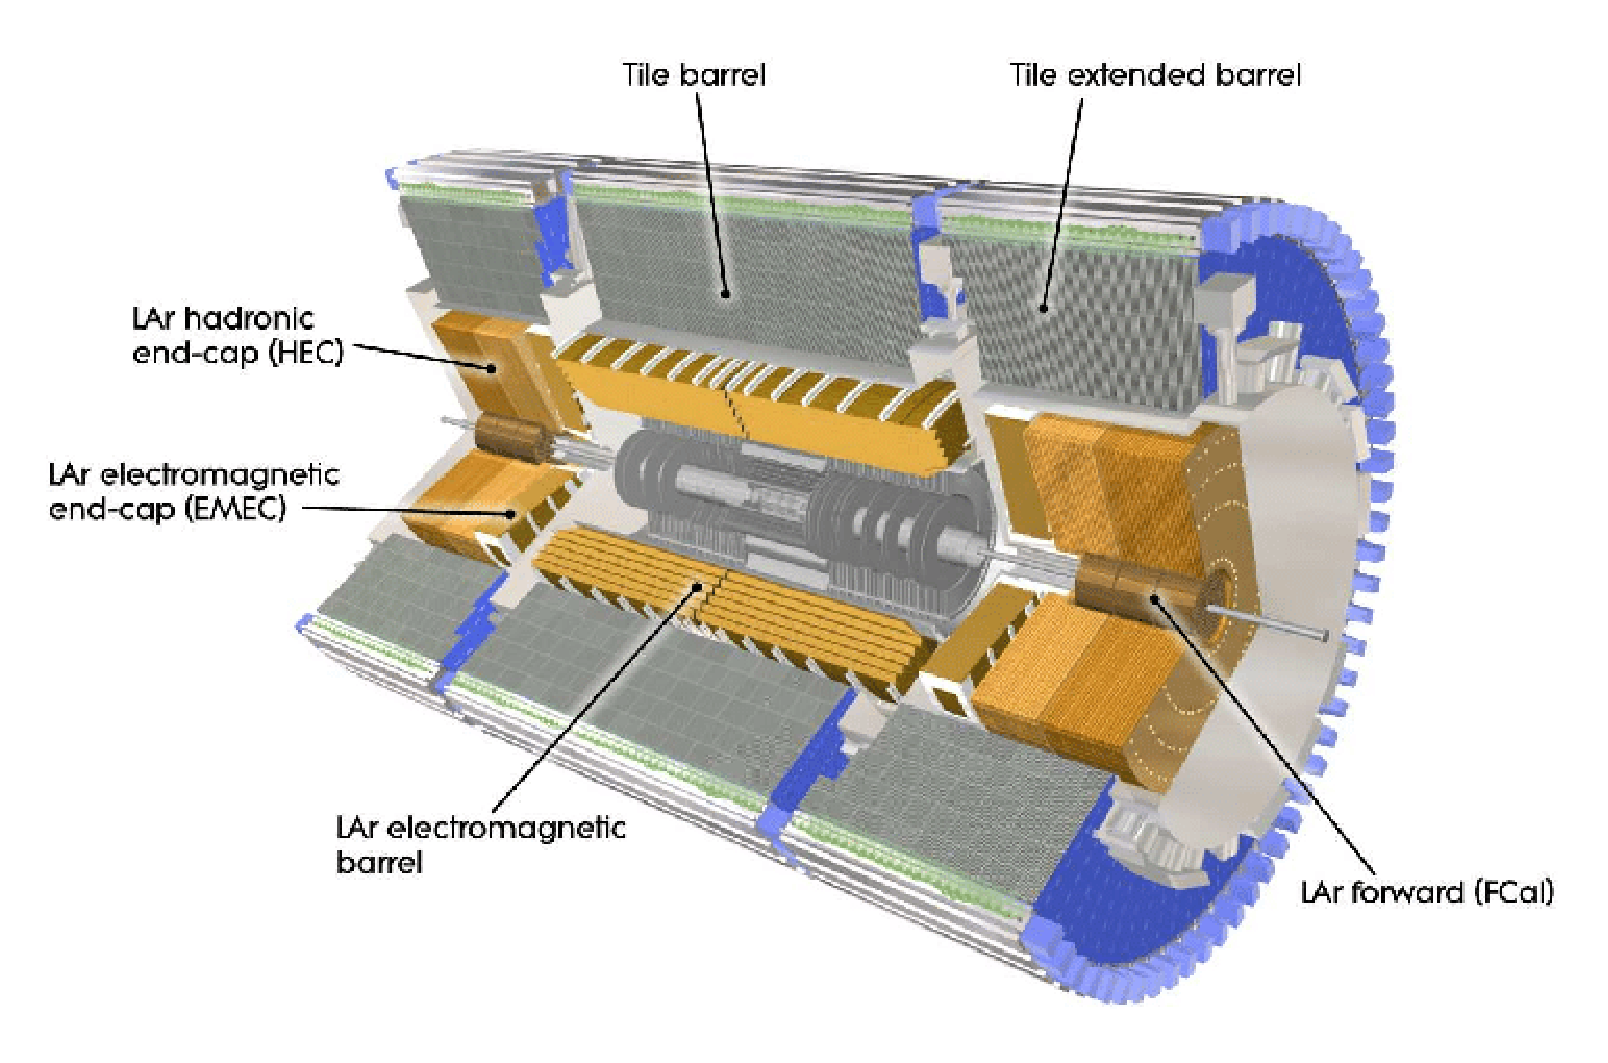
\includegraphics[width=0.9\linewidth]{figures/lhc/calorimeter.eps}
\caption{Cutaway view of the calorimeter system of the ATLAS detector \cite{caloFig}.}
\label{fig:calo}
\end{figure}

Situated outside the Innder Detector are two concentric calorimeters. The inner calorimeter uses liquid argon (LAr) to measure energy of particles the interact electromagnetically, which includes photons and any charged particle. The LAr calorimeter is made of heavy metals, primarily lead and copper, which causes electromagnetically interacting particles to shower, depositing their energy in the detector. The showering of the high energy particles that pass through calorimeter cause the liquid argon to ionize, and the ionized electrons are detected by electronic readouts. The LAr calorimeter consists of around 180,000 readout channels.  

The outer calorimeter measures the energy from particles that pass through the EM calorimeter, and measures the energy of particles that interact via the strong force. This is primarily hadrons. It is composed of steel plates to cause hadronic showering and scintillating tiles as the active material. The signals from the hadronic calorimeter are read out by photomultiplier tubes (PMTs).

\subsection{Muon Spectrometer}
\label{sec:muonSpec}

Because muons are heavier than electrons and photons, and do not interact via the strong force, they generally pass through the detector without being stopped by the calorimeters. The outermost components of the detector are designed specifically to measure the energy and momentum of muons produced in the LHC. The muon spectrometer consists of tracking and triggering system. It extends from the outside of the calormeter system, about a 4.25 m radius from the beam line, to a radius of 11 m. This large detector system is necessary to accurately measure the momentum of muons, which is essential not only for measurements involving the muons themselves, but also to accurately estimate the missing energy in each event.

Two large toroidal magnets within the muon system generate a large magnetic field which covers an area 26 m long with a radius of 10 m. Because the area covered by this magnet system is so large, a uniform magnetic field like the one produced in the Inner Detector is impractical. Instead, the magnetic field that exists in the muon spectrometer ranges between 2 T and 8 T, and is much less uniform. The path of the muons passing through the spectrometer is bent by this field, allowing their charge to be determined. 

1200 tracking chambers are placed in the muon system in order to precisely measure the tracks of muons with high spatial resolution.

%\subsection{Forward Detector}
%\label{sec:forwardDet}

\subsection{Trigger System}
\label{sec:trigger}

Because of the high collision rate and large amount of data collected by the various subdetectors, ATLAS produces far more data than can actually be stored. Each event produces around 25 Mb of raw data, which multiplied by the bunch crossing rate of 40 MHz, comes out to around a petabyte of data every second. The information from every event cannot practically be stored, therefore a sophisticated trigger system is employed in real time to determine whether events are sufficiently interesting to be worth storing.

The trigger system in ATLAS involves multiple levels, each of which select out which events move on to the next level of scrutiny. The level-1 trigger uses hardware information from the calorimeters and muon spectrometer to select events that contain candidates for particles commonly used in analysis, such as energetic leptons and jets. The level-1 trigger reduces the rate of events from 40 MHz to around 100 kHz. 

Events that pass the level-1 trigger move to the High-Level Trigger (HLT). The HLT takes place outside of the detector in software, and looks for properties such as a large amount of missing transverse energy, well defined leptons, and multiple high energy jets. Events that pass the HLT are stored and used for analysis. Because the specifics of the HLT are determined by software rather than hardware, the thresholds can be changed throughout the run of the detector in response to run conditions such as changes to pilup and luminosity. After the HLT is applied, the event rate is reduced to around 1000 per second, which are recorded for analysis.

%-------------------------------------------------------------------------------

%-------------------------------------------------------------------------------
\section{Data and Monte Carlo Samples}
\label{sec:dataMC}
This study used data collected by the ATLAS detector over the period from 2015-2018, representing 138.9 $fb^{-1}$ of data at an energy of 13 TeV. 

Several Monte Carlo generators were used to simulate both signal and background processes. For all of these, the effects of the ATLAS detector are simulated in Geant4. 
%-------------------------------------------------------------------------------

%-------------------------------------------------------------------------------   
\section{Object Reconstruction}
\label{sec:objReco}

All analysis channels considered in this note share a common object selection for leptons and jets, as well as a shared trigger selection. 

\subsection{Trigger Requirements}

Events are required to be selected by dilepton triggers, as summarized in table \ref{tbl:trigger}.

\begin{table}[h!]
 \begin{center}
   \begin{tabular}{cc}
     \toprule
                  & Dilepton triggers (2015) \\
     \midrule
      $\mu\mu$ (asymm.)          & \verb!HLT_mu18_mu8noL1! \\
      $ee$ (symm.)               & \verb!HLT_2e12_lhloose_L12EM10VH! \\
      $e\mu,\mu e$ ($\sim$symm.) & \verb!HLT_e17_lhloose_mu14! \\
     \bottomrule
                       & Dilepton triggers (2016) \\
     \midrule
      $\mu\mu$ (asymm.)                   & \verb!HLT_mu22_mu8noL1! \\
      $ee$ (symm.)                        & \verb!HLT_2e17_lhvloose_nod0! \\
      $e\mu,\mu e$ ($\sim$symm.)          & \verb!HLT_e17_lhloose_nod0_mu14! \\
     \bottomrule

                  & Dilepton triggers (2017) \\
     \midrule
      $\mu\mu$ (asymm.)                   & \verb!HLT_mu22_mu8noL1! \\
      $ee$ (symm.)                        & \verb!HLT_2e24_lhvloose_nod0! \\
      $e\mu,\mu e$ ($\sim$symm.)          & \verb!HLT_e17_lhloose_nod0_mu14! \\
     \bottomrule
                  & Dilepton triggers (2018) \\
     \midrule
      $\mu\mu$ (asymm.)                   & \verb!HLT_mu22_mu8noL1! \\
      $ee$ (symm.)                        & \verb!HLT_2e24_lhvloose_nod0! \\
      $e\mu,\mu e$ ($\sim$symm.)          & \verb!HLT_e17_lhloose_nod0_mu14! \\
      \bottomrule
   \end{tabular}
   \caption{\label{tbl:trigger} List of lowest $p_{T}$-threshold, un-prescaled dilepton triggers used for 2015-2018 data taking.}
 \end{center}
\end{table}

\subsection{Light Leptons}
\label{subsec:lepSelection}

Electron candidates are reconstructed from energy clusters in the electromagnetic calorimeter that are associated with charged particle tracks reconstructed in the inner detector \cite{ATLAS-CONF-2016-024}.  Electron candidates are required to have $\pt > 10$ GeV and $|\eta_\textrm{cluster}| < 2.47$. Candidates in the transition region between different electromagnetic calorimeter components, $1.37 < |\eta_\textrm{cluster}| < 1.52$, are rejected. A multivariate likelihood discriminant combining shower shape and track information is used to distinguish prompt electrons from nonprompt leptons, such as those originating from hadronic showers. 

To further reduce the non-prompt contribution, the track of each electron is required to originate from the primary vertex; requirements are imposed on the transverse impact parameter significance ($|d_0|/\sigma_{d_0}$) and the longitudinal impact parameter ($|\Delta z_0 \sin \theta_\ell|$), as shown in table \ref{tbl:tightleps}.

Muon candidates are reconstructed by combining inner detector tracks with track segments or full tracks in the muon spectrometer \cite{PERF-2014-05}. Muon candidates are required to have $\pt > 10$~GeV and $|\eta| < 2.5$. All leptons are required to be isolated, and pass a non-prompt BDT selection described in detail in \cite{ttH_paper}.

\subsection{Jets}
\label{subsec:jetSelection}

%UPDATE TO PFLOW
Jets are reconstructed from calibrated topological clusters built from energy deposits in the calorimeters \cite{ATL-PHYS-PUB-2015-015}, using the anti-$k_t$ algorithm with a radius parameter $R=0.4$.  Jets with energy contributions likely arising from noise or detector effects are removed from consideration \cite{ATLAS-CONF-2015-029}, and only jets satisfying $\pt > 25$~GeV and $|\eta| < 2.5$ are used in this analysis.  For jets with $\pt < 60$~GeV and $|\eta| < 2.4$, a jet-track association algorithm is used to confirm that the jet originates from the selected primary vertex, in order to reject jets arising from pileup collisions \cite{PERF-2014-03}. 

\subsection{Missing Transverse Energy}

Because all $t\bar{t}H-ML$ channels considered include multiple neutrinos, missing transverse energy ($E_T^{miss}$) is present in each event. The missing transverse momentum vector is defined as the inverse of the sum of the transverse momenta of all reconstructed physics objects as well as remaining unclustered energy, the latter of which is estimated from low-\pt tracks associated with the primary vertex but not assigned to a hard object \cite{ATL-PHYS-PUB-2015-027}.

%------------------------------------------------------------------------------- 

%------------------------------------------------------------------------------- 
\section{Higgs Momentum Reconstruction}
\label{sec:mva}
Reconstructing the momentum of the Higgs boson is a particular challenge for channels with leptons in the final state: Because all channels include at least two neutrinos in the final state, the Higgs can never be fully reconstructed. However, the momentum spectrum can be well predicted by a neural network when provided with the four-vectors of the Higgs Boson decay products, as shown in section \ref{sec:truthLevelReco}. With this in mind, a sophisticated approach involving several layers of MVAs is used to reconstruction the Higgs momentum. 

The first layer is a Neural Network designed to select which jets are most likely to be the b-jets that came from the top decay. The kinematics of these jets are fed into the second layer, also a BDT, which is designed to identify the decay products of the Higgs Boson itself. The kinematics of these particles are then fed into a deep neural-network, which predicts the momentum of the Higgs.

\subsection{Truth Level Reconstruction}
\label{sec:truthLevelReco}

Machine Learning algorithms are trained to identify the decay products of the Higgs Boson using MC simulations of $t\bar{t}H$ events. Reconstructed physics objects are matched to truth level particles, in order to identify the parents of these reconstructed objects. 

\subsection{b-jet Identification}
\label{sec:bjetID}

In both the 3l and 2lSS channels, one or b-tagged jet is required. Therefore, for events which have exactly one, or more than two, b-tagged jets, deciding which combination of jets correspond to the top decay

\subsection{Higgs Reconstruction}
\label{sec:higgsID}

Techniques similar to the b-jet identification algorithms are employed to select the decay products of the Higgs. 

\subsection{$p_T$ Prediction}
\label{sec:ptReco}

Once the most probable decay products have been identified, their kinematics are used to reconstruct the momentum spectrum of the Higgs Boson. 

\subsection{3l Decay Mode}
\label{sec:decay3l}

In the 3l channel, there are two possible ways for the Higgs to decay, both involving intermediate W boson pairs: Either both W bosons decay leptonically, in which case the reconstructed decay consists of two leptons (referred as the fully-leptonic 3l channel), or one W decays leptonically and the other hadronically, giving two jets and one lepton in the final state (referred to as the semi-leptonic 3l channel). In order to accurately reconstruct the Higgs, it is necessary to identify which of these decays took place for each 3l event.




%-------------------------------------------------------------------------------

%-------------------------------------------------------------------------------
\section{Signal Region Definitions}
\label{sec:signal_region}
Events are divided into two channels based on the number of leptons in the final state: one with two same-sign leptons, the other with three leptons. The $3l$ channel includes events where both leptons originated from the Higgs boson as well as events where only one of the leptons 

%------------------------------------------------------------------------------------------

\subsection{Pre-MVA Event Selection}
\label{subsec:preMVA}

A preselection is applied to define orthogonal analysis channels based on the number of leptons in each event. For the 2lSS channel, the following presection is used:

\begin{itemize}
  \item Two very tight, same-charge, light leptons with $p_T > 20$ GeV
  \item $>=$4 reconstructed jets, $>=$1 b-tagged jets
  \item No reconstructed tau candidates
\end{itemize}

\begin{figure}[h!]
    \subfigure[]{\includegraphics[width=.29\linewidth]{trexPlots/stat2l_80/Plots/lep_Pt_0.png}}%                        
    \subfigure[]{\includegraphics[width=.29\linewidth]{trexPlots/stat2l_80/Plots/lep_Pt_1.png}}%                     
    \subfigure[]{\includegraphics[width=.29\linewidth]{trexPlots/stat2l_80/Plots/Mll01}}\\
    \subfigure[]{\includegraphics[width=.29\linewidth]{trexPlots/stat2l_80/Plots/nJets.png}}%                       
    \subfigure[]{\includegraphics[width=.29\linewidth]{trexPlots/stat2l_80/Plots/nbJets.png}}%                
    \subfigure[]{\includegraphics[width=.29\linewidth]{trexPlots/stat2l_80/Plots/MET.png}}\\
    \caption{}                           
    \label{fig:presel2lSS}
\end{figure}

For the 3l channel, the following selection is applied:

\begin{itemize}
  \item Three light leptons with total charge $\pm 1$
  \item Same charge leptons are required to be very tight, with $p_T > 20$ GeV
  \item Opposite charge lepton must be loose, with $p_T > 10$ GeV
  \item $>=$2 reconstructed jets, $>=$1 b-tagged jets                                                                        
  \item No reconstructed tau candidates
  \item $|M(l^+l^-)-91.2\textrm{ GeV}| > 10$~\GeV{} for all opposite-charge, same-flavor lepton pairs
\end{itemize}

\begin{figure}[h!]
    \subfigure[]{\includegraphics[width=.29\linewidth]{trexPlots/stat3l_80/Plots/lep_Pt_0.png}}%                             
    \subfigure[]{\includegraphics[width=.29\linewidth]{trexPlots/stat3l_80/Plots/lep_Pt_1.png}}%                      
    \subfigure[]{\includegraphics[width=.29\linewidth]{trexPlots/stat3l_80/Plots/Mll01}}\\                             
    \subfigure[]{\includegraphics[width=.29\linewidth]{trexPlots/stat3l_80/Plots/nJets.png}}%                          
    \subfigure[]{\includegraphics[width=.29\linewidth]{trexPlots/stat3l_80/Plots/nbJets.png}}%                          
    \subfigure[]{\includegraphics[width=.29\linewidth]{trexPlots/stat3l_80/Plots/MET.png}}\\                         
    \caption{}
    \label{fig:presel3l}                                                                                          
\end{figure}

%------------------------------------------------------------------------------------------

\subsection{Event MVA}
\label{subsec:sigBkgMVA}

Separate multi-variate analysis techniques (MVAs) are used in order to distinguish signal events from background for each analysis channel - 2lSS, 3l semi-leptonic, and 3l fully leptonic. In particular, Neural Networks produced with Tensorflow are trained using the kinematics of signal and background events derived from Monte Carlo simulations. Further, because the background composition differs for events with a high reconstructed Higgs $p_T$ compared to events with low reconstructed Higgs $p_T$, separate MVAs are produced for high and low $p_T$ regions.

Output distributions of each MVA are shown in figure \ref{fig:sigBkgScore}. Detailed explanations of each of the models can be found in section \ref{apx:MVA}.

\begin{figure}
  \subfigure[]{\includegraphics[width=.3\linewidth]{trexPlots/xgb_higgsDiff/Plots/xgb_sigBkg_2lHigh.png}}%
  \subfigure[]{\includegraphics[width=.3\linewidth]{trexPlots/xgb_higgsDiff/Plots/xgb_sigBkg_3lSHigh.png}}%
  \subfigure[]{\includegraphics[width=.3\linewidth]{trexPlots/xgb_higgsDiff/Plots/xgb_sigBkg_3lFHigh.png}}\\
  \subfigure[]{\includegraphics[width=.3\linewidth]{trexPlots/xgb_higgsDiff/Plots/xgb_sigBkg_2lLow.png}}%
  \subfigure[]{\includegraphics[width=.3\linewidth]{trexPlots/xgb_higgsDiff/Plots/xgb_sigBkg_3lSLow.png}}%
  \subfigure[]{\includegraphics[width=.3\linewidth]{trexPlots/xgb_higgsDiff/Plots/xgb_sigBkg_3lFLow.png}}
  \label{fig:sigBkgScore}
  \caption{scores}
\end{figure}

%------------------------------------------------------------------------------------------

\subsection{Signal Region Definitions}
\label{subsec:sigRegions}

Once pre-selection has been applied, channels are further refined based on the MVAs described above. The output of the model described in section \ref{sec:decay3l} is used to separate the three channel into two - Semi-leptonic and Fully-leptonic - based on the predicted decay mode of the Higgs boson. 

For each event, depending on the channel as well as the predicted $p_T$ of the Higgs derived from the algorithm described in section \ref{sec:ptReco}, a cut on the appropriate background rejection algorithm is applied. The specific selection used, and the event yield in each channel after this selection has been applied, is summarized below.

\subsubsection{$2lSS$}

\subsubsection{$3l - Semi-leptonic$}

\subsubsection{$3l - Fully-leptonic$}

%-------------------------------------------------------------------------------

%-------------------------------------------------------------------------------
\section{Systematic Uncertainties}
\label{sec:sys}
The systematic uncertainties that are considered are summarized in Table \ref{tab:SystSummary}. These are implemented in the fit either as a normalization factors or as a shape variation or both in the signal and background estimations. The numerical impact of each of these uncertainties is outlined in section \ref{sec:results}.

\begin{table}[H]
\centering
\caption{Sources of systematic uncertainty considered in the analysis. Some of the systematic uncertainties are split into several components, as indicated by the number in the rightmost column.}
\begin{tabular}{lr}
\hline\hline
Systematic uncertainty & Components           \\
\hline
\hline
Luminosity      & 1                   \\
Pileup reweighting      & 1                   \\
\textbf {Physics Objects}       &                     \\
\ \ Electron                                    & 6                   \\
\ \ Muon        & 15                  \\
\ \ Jet energy scale and resolution     & 28                  \\
\ \ Jet vertex fraction         & 1                   \\
\ \ Jet flavor tagging          & 131                 \\
\ \ $E^{miss}_T$        & 3                   \\
\hline
Total (Experimental)        & 186                    \\
\hline
\hline
\textbf {Background Modeling}           &                     \\
\ \ Cross section                       & 24                  \\
\ \ Renormalization and factorization scales    & 10                  \\
\ \ Parton shower and hadronization model               & 2                   \\
\ \ Shower tune                         & 4                   \\
\hline
Total (Signal and background modeling)       & 40                    \\
\hline
\hline
\textbf {Background Modeling}           &                     \\
\ \ Cross section                       & 24                  \\
\ \ Renormalization and factorization scales    & 10                  \\
\ \ Parton shower and hadronization model               & 2                   \\
\ \ Shower tune                         & 4                   \\
\hline
Total (Signal and background modeling)       & 40                    \\
\hline\hline
Total (Overall)                             & 226             \\
\hline\hline
\end{tabular}
\label{tab:SystSummary}
\end{table}

The uncertainty in the combined integrated luminosity is derived from a calibration of the luminosity scale using x-y beam-separation scans performed for 13 TeV proton-proton data \cite{lumi}, \cite{LUCID2}.

The experimental uncertainties are related to the reconstruction and identification of light leptons and and b-tagging of jets, and to the reconstruction of $E^{miss}_T$. 

The sources which contribute to the uncertainty in the jet energy scale \cite{jes} are decomposed into uncorrelated components and treated as independent sources in the analysis. This method decomposes the uncertainties into 30 nuiscance parameters included in the fit. A similar method is used to account for jet energy resolution (JER) uncertainties, and 8 JER uncertainty components are uncluded as NPs in the fit.

The uncertainties in the b-tagging efficiencies measured in dedicated calibration analyses \cite{btag_cal} are also decomposed into uncorrelated components. The large number of components for b-tagging is due to the calibration of the distribution of the BDT discriminant.

As mentioned in Section \ref{sec:MCsamples}, a normalization corrections and uncertainties on the estimates of non-prompt leptons backgrounds are derived using data driven techniques, decribed in detail in \cite{ttH_paper}. These are derived from a likelihood fit over various non-prompt enriched control regions, targeting several sources of non-prompt light leptons separately: external conversion electrons, internal conversion electrons, electrons from heavy flavor decays, and muons from heavy flavor decays. %These are used to derive overall fake factors for electrons from light source (e.g. photon conversions or light hadrons), electrons from heavy flavor decays (namely, charm or bottom hadrons), and a single fake factor for muons.

The normalization factor and uncertainty applied to each source of non-prompt leptons is summarized in Table \ref{tab:fakeNF}

\begin{table}[H]
\begin{center}
\begin{tabular}{c|c}
\hline\hline
Processs &  Normalization Factor\\
\hline
$NF_e^{ExtCO}$ & 1.70 $\pm$ 0.51 \\
$NF_e^{IntCO}$ & 0.75 $\pm$ 0.26 \\
$NF_e^{HF}$ & 1.09 $\pm$ 0.32 \\
$NF_{\mu}^{HF}$ & 1.28 $\pm$ 0.17 \\
\hline
\end{tabular}
\label{tab:fakeNF}
\caption{Normalization factors - with statistical and systematic uncertainties - derived from the fit over fake control regions for each source of non-prompt leptons considered.}
\end{center}
\end{table}


In addition to those derived from the control regions, several additional uncertainties are assigned to the non-prompt lepton background. An additional 25\% uncertainty on material conversions is assigned, based on the comparison between data and MC in a region where a loose electron fails the photon conversion veto. A shape uncertainty of 15\% (6\%) is assigned to the HF non-prompt electron (muon) background based on a comparison between data and MC where the second leading electron (muon) is only required to be loose. As the contribution from light non-prompt leptons is small, about 10\% percent of the contribution from HF non-prompt leptons, it is derived from the agreement between data and simulation in a LF enriched region at low values of the non-prompt lepton BDT. The resulting uncertainty is 100\%, and is taken to be uncorrelated between internal and material conversions.

Theoretical uncertainties applied to MC predictions, including cross section, PDF, and scale uncertainties are taken from theory calculations for the predominate prompt backgrounds. Following the nominal $t\bar{t}H-ML$ analysis, a 50\% uncertainty is applied to Diboson to account for the large uncertainty in estimating VV + heavy flavor. The other ``rare'' background processes - including $tZ$, rare top processes, $ttWW$, $WtZ$, $VVV$, $tHjb$ and $WtH$ - are assigned an overall 50\% normalization uncertainty as well. The theory uncertainties applied to the MC estimates are summarized in Table \ref{tab:xsecUnc}.

\begin{table}[H]                                                                                                              {\footnotesize
\centering
../ttHDiff-PUB-Note/sections/ttH_xsecUnc.tex
\caption{Summary of theoretical uncertainties for MC predictions in the analysis.}
\label{tab:xsecUnc}}
\end{table}

Additional uncertainties to account for $t\bar{t}W$ mismodelling are also applied. These include a ``Generator'' uncertainty, based on a comparison between the nominal Sherpa 2.2.5 sample, and the formerly used aMC@NLO sample, and an ``Extra radiation'' uncertainty, which includes renormalisation and factorisation scale variations of the Sherpa 2.2.5 sample.

%-------------------------------------------------------------------------------

%-------------------------------------------------------------------------------
\section{Results}
\label{sec:results}
Unblinded results are shown for the 80 $fb^{-1}$ data set, as well as MC only projections of results using the full Run-2, 140 $fb^{-1}$ dataset.

%-------------------------------------------
\subsection{Results - 80 $fb^{-1}$}
\label{sec:res80}
%-------------------------------------------

A maximum likelihood fit is performed simultaneously over the regions shown in figure \ref{fig:sigRegions80}.

\begin{figure}[h!]
    \subfigure[]{\includegraphics[width=.29\linewidth]{trexPlots/stat_80/Plots/recoHiggsPt_2lSS_postFit.png}}%   
    \subfigure[]{\includegraphics[width=.29\linewidth]{trexPlots/stat_80/Plots/recoHiggsPt_3lS_postFit.png}}%    
    \subfigure[]{\includegraphics[width=.29\linewidth]{trexPlots/stat_80/Plots/recoHiggsPt_3lF_postFit.png}}\\
    \caption{}
    \label{fig:sigRegions80}
\end{figure}

\begin{figure}[h!]
    \center
    \includegraphics[width=.9\linewidth]{trexPlots/stat_80/Plots/Summary_postFit.png}
    \caption{Post-fit summary of fit.}                                                                          
    \label{fig:Summary80}
\end{figure}

\begin{figure}[H]
    \centering
    \includegraphics[width=0.7\linewidth]{trexPlots/stat_80/PieChart_postFit.png}
    \caption{Background composition of the fit regions.}
    \label{fig:pieChart80}
\end{figure} 

%-------------------------------------------

%-------------------------------------------                                                                                 
\subsection{Projected Results - 140 $fb^{-1}$}   
\label{sec:res140}
%------------------------------------------- 

\begin{figure}[h!]
    \subfigure[]{\includegraphics[width=.29\linewidth]{trexPlots/stat_140/Plots/recoHiggsPt_2lSS_postFit.png}}%             
    \subfigure[]{\includegraphics[width=.29\linewidth]{trexPlots/stat_140/Plots/recoHiggsPt_3lS_postFit.png}}%        
    \subfigure[]{\includegraphics[width=.29\linewidth]{trexPlots/stat_140/Plots/recoHiggsPt_3lF_postFit.png}}\\
    \caption{}
    \label{fig:sigRegions140}
\end{figure}

\begin{figure}[h!]
    \center
    \includegraphics[width=.9\linewidth]{trexPlots/stat_140/Plots/Summary_postFit.png}
    \caption{Post-fit summary of fit.}
    \label{fig:Summary140}
\end{figure}

\begin{figure}[H]
    \centering                                                                                                               
    \includegraphics[width=0.7\linewidth]{trexPlots/stat_140/PieChart_postFit.png}
    \caption{Background composition of the fit regions.}
    \label{fig:pieChart140}
\end{figure}

%-------------------------------------------

%------------------------------------------------------------------------------

%-------------------------------------------------------------------------------
\section{Conclusion}
\label{sec:conclusion}

As search for the effects of dimension-six operators on $t\bar{t}H$ production is performed. An effective field theory approached is used to parameratize the effects of high energy physics on the Higgs momentum spectrum. The momentum spectrum is reconstructed using various MVA techniques, and the limits on dimension-six operators are limited to X. 


%-------------------------------------------------------------------------------
% If you use biblatex and either biber or bibtex to process the bibliography
% just say \printbibliography here
\printbibliography
% If you want to use the traditional BibTeX you need to use the syntax below.
%\bibliographystyle{bib/bst/atlasBibStyleWithTitle}
%\bibliography{wz_heavy_flavor,bib,ATLAS,bib/CMS,bib/ConfNotes,bib/PubNotes}
%-------------------------------------------------------------------------------

%-------------------------------------------------------------------------------
% Print the list of contributors to the analysis
% The argument gives the fraction of the text width used for the names
%-------------------------------------------------------------------------------
\clearpage
\PrintAtlasContribute{0.30}


%-------------------------------------------------------------------------------
\clearpage
\appendix
\part*{Appendices}
\addcontentsline{toc}{part}{Appendices}
%-------------------------------------------------------------------------------

\subsection{Non-prompt lepton MVA}
\label{sec:lepMVA}
\input{sections/lepMVA}

%-------------------------------------------------------------------------------
\section{Machine Learning Models}
\label{apx:MVA}

The following section provides details regarding the various machine learning models used in the analysis. The Keras neural network framework, with Tensorflow as the backend, is used to create each model, and the number of hidden layers and nodes are determined using grid search optimization. For each model, a LeakyReLU activation function is used, along with a learning rate of 0.01, and the Adam optimization algorithm. For the classification algorithms (b-jet matching, Higgs reconstruction, and background separation) binary-cross entropy is used as the loss function. 

\subsection{b-jet Identification Algorithms}
\label{subsec:higgsRecoMVA}

%---------------------------------------------------------------------- 
\subsubsection{2lSS Channel}
\label{subsec:Apptop2lSS}
%---------------------------------------------------------------------- 
                                                                                                                     
For the 2lSS channel, the following input features as used for training:

%----------------------------------------------------------------------
\subsubsection{3l Channel}
\label{subsec:top3l}
%---------------------------------------------------------------------- 


%----------------------------------------------------------------------

\subsection{Higgs Reconstruction Algorithms}
\label{subsec:higgsRecoMVA}

%----------------------------------------------------------------------                                                    
\subsubsection{2lSS Channel}
\label{subsec:higgs2lSS}
%----------------------------------------------------------------------  



%----------------------------------------------------------------------

%----------------------------------------------------------------------                                                   
\subsubsection{3l Semi-leptonic Channel}
\label{subsec:higgs3lS}
%----------------------------------------------------------------------  



%----------------------------------------------------------------------

%----------------------------------------------------------------------                                                    
\subsubsection{3l Fully-leptonic Channel}                                  
\label{subsec:higgs3lF}                                                                                                   
%----------------------------------------------------------------------



%----------------------------------------------------------------------

\subsection{$p_T$ Prediction MVA}
\label{subsec:ptMVA}

%----------------------------------------------------------------------                                                  
\subsubsection{2lSS Channel}                                                                          
\label{subsec:pt2lSS}                                                                                           
%----------------------------------------------------------------------                                                     



%----------------------------------------------------------------------
 
%----------------------------------------------------------------------                                                  
\subsubsection{ 3l Semi-leptonic Channel}                                                                            
\label{subsec:pt3lS}                                                                                                    
%----------------------------------------------------------------------                                                      



%----------------------------------------------------------------------
 
%----------------------------------------------------------------------                                                
\subsubsection{ 3l Fully-leptonic Channel}                                                                            
\label{subsec:pt3lF}                                                                                                    
%----------------------------------------------------------------------



%----------------------------------------------------------------------

%----------------------------------------------------------------------
\subsection{3l Decay MVA}
\label{subsec:decayMVA}
%----------------------------------------------------------------------



%----------------------------------------------------------------------

%-------------------------------------------------------------------------------

\end{document}
